\documentclass[conference]{IEEEtran}
\usepackage[utf8]{inputenc}
\usepackage[T1]{fontenc}
\usepackage{cite}
\usepackage{amsmath,amssymb}
\usepackage{graphicx}
\usepackage{booktabs}
\usepackage{array}
\usepackage{url}
\usepackage{xcolor}
\usepackage[hidelinks]{hyperref}
\newcommand{\ft}[1]{\texttt{\detokenize{#1}}}
\newcommand{\todo}[1]{\textbf{[TODO: #1]}}
\newcommand{\verify}{\textbf{[VERIFY]}}
\makeatletter
\newcommand{\linebreakand}{%
  \end{@IEEEauthorhalign}
  \hfill\mbox{}\par
  \mbox{}\hfill\begin{@IEEEauthorhalign}
}
\makeatother
\graphicspath{{./}}

\begin{document}

\title{How Much of Malicious-Document Detection Accuracy Is Real?\\An Audit of CIC-Trap4Phish}

% \author{\IEEEauthorblockN{\todo{author names}}
% \IEEEauthorblockA{\todo{affiliation, e-mail}}}
\author{
\IEEEauthorblockN{Atharv Kulkarni}
\IEEEauthorblockA{Walchand College of Engineering, Sangli, India}
\and
\IEEEauthorblockN{Bhargav Joshi}
\IEEEauthorblockA{Walchand College of Engineering, Sangli, India}
\linebreakand
\IEEEauthorblockN{Hrushikesh Jadhav}
\IEEEauthorblockA{Walchand College of Engineering, Sangli, India}
\linebreakand
\IEEEauthorblockN{Manisha Dabade}
\IEEEauthorblockA{Walchand College of Engineering, Sangli, India}
\and
\IEEEauthorblockN{Dr. Pawan Kumar}
\IEEEauthorblockA{Indian Institute of Information Technology Dharwad, India}
}

\maketitle

\begin{abstract}
Public static-feature benchmarks for malicious-document detection report near-perfect scores, but duplicates, collection artifacts and shortcut features may inflate them. We audit the CIC-Trap4Phish 2025 benchmark (Word, Excel, PDF, HTML) with three evaluation levels: a naive split (L0), exact deduplication (L1), and deduplication with shortcut and missing-value columns removed (L2). Between 22.8\% and 33.0\% of rows lie in exact-duplicate groups, and 20.9--32.9\% of L0 test rows have an exact feature twin in training. On HTML, a tuned LightGBM scores F1 0.857 [0.840, 0.873] on non-twin test rows versus 0.986 on twin rows. Word F1 falls from 1.000 (L1) to 0.937 [0.929, 0.945] (L2) after 41 of 43 columns are removed; Excel remains perfectly separable without macro and API columns, consistent with synthetic benign files. Deduplication alone does not lower F1 in every format. A pooled format-agnostic model trails specialists by 0.009 [0.006, 0.013] F1 on PDF and 0.073 [0.060, 0.085] on HTML, with the per-format HTML gap shrinking as the feature budget grows. We give recommendations for building static malicious-document benchmarks.
\end{abstract}

\begin{IEEEkeywords}
malicious documents, static analysis, benchmark audit, data leakage, shortcut learning, feature generalization
\end{IEEEkeywords}

\section{Introduction}
Machine-learning detectors for malicious office, PDF and HTML documents are commonly evaluated on public tabular benchmarks of static features. CIC-Trap4Phish 2025 \cite{nejati2026} provides such features for four formats, and reported macro-F1 values are close to saturation for Word, Excel and PDF. Saturated scores on a public benchmark invite a question that the machine-learning security literature has raised repeatedly \cite{arp2022,kapoor2023,allamanis2019,geirhos2020}: how much of the reported accuracy reflects the detection task, and how much reflects duplicates, collection artifacts and shortcut features?

Prior work on this release trains on the data as distributed. Sen and Chowdhury \cite{sen2026} pool all four formats into one zero-filled union without deduplication, and Ayodeji et al.\ \cite{ayodeji2026} study PDF only; to our knowledge neither reports a duplicate or provenance analysis. We therefore ask (i) how much of the accuracy survives deduplication and shortcut removal, (ii) what the honest per-format performance is, and (iii) whether a small format-agnostic feature set can replace per-format feature sets.

\textbf{Contributions.} We do not propose a new detector or dataset and make no state-of-the-art claim. Our contributions are:
\begin{itemize}
\item \textbf{C1} A measured audit of the benchmark: exact duplicate feature vectors, train/test ``twin'' leakage in naive splits, provenance confounds, and single-feature shortcuts, in all four formats.
\item \textbf{C2} A three-level evaluation protocol (L0 naive split, L1 deduplicated, L2 deduplicated with shortcut and missing-value columns removed) and an ``honest leaderboard'' with bootstrap confidence intervals.
\item \textbf{C3} A format-agnostic (``universal'') feature study with a pooled model, a feature-budget sensitivity analysis, and a comparison of shortcut-bearing and shortcut-free Word adapters.
\item \textbf{C4} An analysis of the zero-filled union representation used by prior work (SHAP share on own-format versus other-format columns), plus leave-one-format-out transfer.
\item \textbf{C5} Recommendations for building and evaluating static malicious-document benchmarks, and a reproducible release (code, seeds, split indices).
\end{itemize}

\section{Related Work and Dataset}
\subsection{Prior results on this benchmark}
Table~\ref{tab:prior} summarizes the setups of prior work. Sen and Chowdhury \cite{sen2026} report 98.45\% test accuracy for a random forest (their Table~I; 0.9839 in Table~IV and 98.39\% in Table~V) on an 8-class zero-filled union of $N=79{,}293$ rows, the sum of the four raw files, with an 80/20 split; errors concentrate in HTML. Ayodeji et al.\ \cite{ayodeji2026} compare an MLP and a TabTransformer on 3--4 selected PDF features (19,296 samples) and report 97.7\% accuracy at 5k samples. The dataset paper \cite{nejati2026} uses 70/30 splits with the top-10 (top-13 for HTML) selected features and reports macro-averaged F1 of 1.000 (Word), 0.9995--0.9997 (Excel), 0.993--0.9964 (PDF) and 0.911--0.9385 (HTML). These numbers are not directly comparable to ours because splits, class definitions, feature sets, deduplication and metrics differ (Table~\ref{tab:prior}); we do not claim that any of them is wrong, only that the items listed under ``dedup'' were not reported.

\begin{table*}[t]
\centering\footnotesize
\caption{Evaluation setups of prior work and this study; cross-paper scores are not directly comparable. Entries for prior work follow the published papers; ``--'' means not reported or not described.}
\label{tab:prior}
\begin{tabular}{p{2.6cm}p{2.6cm}p{1.7cm}p{3.0cm}p{1.6cm}p{3.6cm}}
\toprule
Work & Scope & Split & Features & Dedup. & Reported metric \\
\midrule
Sen \& Chowdhury \cite{sen2026} & 8-class zero-filled union, $N=79{,}293$ (sum of raw files) & 80/20 & Zero-filled union of all columns & None (raw files) & RF accuracy 98.45\% (Table~I), 0.9839 (Table~IV), 98.39\% (Table~V) \\
Ayodeji et al.\ \cite{ayodeji2026} & PDF only, 19,296 samples & -- & 3--4 selected features & -- (not described) & 97.7\% accuracy at 5k samples (MLP vs.\ TabTransformer) \\
Nejati et al.\ \cite{nejati2026} & Four formats (dataset paper) & 70/30 & Top-10 (top-13 for HTML) selected & -- & Macro-F1 per format (see text) \\
Lu et al.\ \cite{lu2021} & Universal static detection: PDF, Word, Excel, RTF and image documents; two datasets & -- (not stated in abstract) & Generalized features: specification-check errors, structure path, code keywords, object counts & -- (not stated in abstract) & Average F1 0.99 (abstract) \\
This study & Four formats, per-format and pooled & Stratified 80/20, seed 42 & All columns; 10 format-agnostic slots & Exact (L1, L2) & F1 with 95\% bootstrap CI \\
\bottomrule
\end{tabular}
\end{table*}

\subsection{Format-agnostic detection}
Lu et al.\ \cite{lu2021} study universal static detection of malicious documents through feature generalization and are, to our knowledge, the closest prior work on format-agnostic features. Our study differs in three respects: it is an audit of a public benchmark release, it adds a pooled cross-format model evaluated with paired significance tests, and it compares shortcut-bearing with shortcut-free adapters.

\subsection{Dataset provenance}
The dataset paper \cite{nejati2026} reports 20,000 samples per format. The released feature files used here contain 20,000 Word rows with 43 features, 20,000 Excel rows with 48, 19,296 PDF rows with 40 and 19,997 HTML rows with 40. According to the dataset paper, the 10,000 benign Excel files were generated synthetically; benign Word and HTML files were crawled (Google, Wikipedia, PhishTank); malicious Word and Excel files come from MalwareBazaar; PDF files come from PDFMal2022; and malicious HTML comes from PhishTank. Benign and malicious classes therefore come from different sources for Word, Excel and HTML, which creates the provenance confounds examined below.

\section{Audit and Evaluation Protocol}
\textbf{Levels.} L0 is the raw data with a stratified 80/20 split (seed 42). L1 removes exact duplicate feature vectors (keep-first) and, for HTML, six feature vectors that occur with both labels, before an identical split. L2 additionally removes (a) columns with missing values in the raw data and (b) columns whose single-feature decision-stump accuracy, estimated by 5-fold cross-validation on the L1 training split, is at least 0.95. We always name two quantities separately: \emph{rows inside duplicate groups} and \emph{rows removed by keep-first deduplication}.

\textbf{Twin leakage.} A test row is a \emph{twin} if an identical feature vector occurs in the training set of the same split. We report the twin share at L0 and compare accuracy and F1 on twin and non-twin test rows for one fitted model.

\textbf{Provenance and shortcuts.} We fit a depth-1 decision tree on the integer-coded folder name (or lowercase file extension) of each file and report its accuracy on all rows; the path is never used as a model feature. The Word release has no path field, so provenance could not be assessed for Word. Shortcut screening uses 5-fold cross-validated decision-stump accuracy on each feature, and for Word also on missing-value indicators.

\textbf{Models and statistics.} Five model families are tuned per cell: LightGBM \cite{ke2017} 4.7.0, XGBoost 3.2.0, Random Forest, Decision Tree and Logistic Regression (scikit-learn 1.7.2), using Optuna \cite{akiba2019} 5.0.0 (TPE sampler, seed 42, 8 trials; objective: mean F1 at threshold 0.5 over 3-fold stratified inner CV on the training split only); the reporting threshold is chosen on out-of-fold predictions. The specialist reported in Table~\ref{tab:lb} is the tuned LightGBM. Test F1 comes with 95\% bootstrap confidence intervals \cite{efron1979} (2000 resamples). Paired comparisons use the Nadeau--Bengio corrected resampled $t$-test \cite{nadeau2003} on $5\times5$ repeated CV ($J=25$, 24 degrees of freedom), McNemar's test \cite{mcnemar1947}, Holm correction \cite{holm1979} and Cohen's $d$.

\textbf{Universal features.} Ten format-agnostic feature slots (e.g., content entropy, active-content flag, log file size, embedded-object count) are mapped to each format by hand-designed adapters (\ft{mapping_log.json}); the external-reference slot has no Word counterpart and is a constant 0. A \emph{per-format} universal model uses slots 1 to $k$, $k\in\{4,6,8,10\}$, in numeric order. A \emph{pooled} model is a single LightGBM trained on the L1 training splits of all four formats mapped to the first six slots ($k=6$). In all comparisons $\Delta F1$ is specialist F1 minus universal F1; the specialist is the tuned LightGBM trained on all columns available at the stated level (L1; L2 for ``Word (no shortcuts)'').

\textbf{Zero-filled union and explanation.} In the zero-filled union (Arm~4), the columns of all four formats are concatenated and missing columns are zero-filled; the model is a LightGBM on the binary label. We use TreeSHAP \cite{lundberg2017} on the first 200 test rows of each format and report the share of mean $|$SHAP$|$ on a row's own-format columns. Leave-one-format-out (LOFO) trains on three formats with the first six universal slots and tests on the fourth; its specialist baseline is the format's L1 specialist. On the HTML errors we also run LIME \cite{ribeiro2016} (500 samples, 5 features) and permutation importance (5 repeats).

\section{Results}
\subsection{Audit findings}
\textbf{Duplicates.} Table~\ref{tab:audit} shows that 22.8\% (Word) to 33.0\% (Excel) of rows lie inside exact-duplicate groups. Duplicates are strongly label-skewed: all 4,558 Word duplicate rows are benign, all 6,591 Excel duplicate rows are malicious, PDF has 28 benign and 5,675 malicious, and HTML 434 benign and 5,249 malicious. Deduplication therefore changes the class balance as well as the test set. Six HTML feature-vector groups occur with both labels and were removed.

\textbf{Twin leakage.} At L0, 20.9\% (834/4,000) of Word, 32.9\% (1,314/4,000) of Excel, 27.8\% (1,074/3,860) of PDF and 27.1\% (1,083/4,000) of HTML test rows have an exact twin in training.

\textbf{Provenance.} The folder name predicts the label with accuracy 1.000 in Excel, PDF and HTML; the Word release has no path field, so Word could not be tested. The file extension alone gives 0.631 for Excel, 0.518 for PDF and 0.500 for HTML (Table~\ref{tab:audit}).

\textbf{Shortcuts.} In Word, 30 of the 43 feature columns are missing in exactly 10,000 of 20,000 rows; 22 are missing only for benign files and 8 only for malicious files, so each missing-value indicator separates the classes with stump accuracy 1.000. Of the 43 Word columns, 19 have stump accuracy $\ge0.95$, including \ft{ole_object_count}, \ft{ole_object_type_count} and \ft{vba_keywords_count} at 1.000; \ft{ole_object_count} is 0 for every benign file and between 11 and 100 for every malicious file. Excel has nine such columns; the strongest are \ft{entropy_of_text} (0.987), \ft{macro_chr_count} (0.985), \ft{macro_token_count} and \ft{macro_vocab_size} (0.980 each), and \ft{macro_arithmetic_operator_count} (0.975), see Fig.~\ref{fig:stump}. No PDF or HTML column reaches 0.95 (maxima 0.929 and 0.788). L2 therefore removes 41 of 43 Word columns (30 with missing values, 11 more by the stump rule) and nine of 48 Excel columns; only \ft{struct_typeface} and \ft{struct_script} remain for Word. Fig.~\ref{fig:erosion} shows that removing features one at a time in order of stump accuracy barely changes Word or Excel F1: the shortcuts are redundant, so single removals do not expose them. All ten of the dataset paper's published top-10 Word features and seven of its ten Excel features are among the columns flagged here \cite{nejati2026}.

\begin{table*}[t]
\centering\footnotesize
\caption{Audit summary (\texttt{audit\_duplicates.csv}, \texttt{audit\_twin\_leakage.csv}, \texttt{audit\_provenance.csv}). ``In groups'' counts rows inside exact-duplicate groups; ``Removed'' counts rows removed by keep-first deduplication (HTML: plus six conflicting-label vectors). Twin share is measured on the L0 test set. Last column: label accuracy from folder name / from file extension (n/a for Word: the release has no path field).}
\label{tab:audit}
\begin{tabular}{lrrrrrrr}
\toprule
Format & Rows & In groups & Dup. ben./mal. & Removed & L1 rows & L0 twin share & Folder/ext. acc. \\
\midrule
Word & 20,000 & 4,558 (22.8\%) & 4,558/0 & 3,395 & 16,605 & 20.9\% (834/4,000) & n/a \\
Excel & 20,000 & 6,591 (33.0\%) & 0/6,591 & 6,028 & 13,972 & 32.9\% (1,314/4,000) & 1.000/0.631 \\
PDF & 19,296 & 5,703 (29.6\%) & 28/5,675 & 3,943 & 15,353 & 27.8\% (1,074/3,860) & 1.000/0.518 \\
HTML & 19,997 & 5,683 (28.4\%) & 434/5,249 & 4,587 (+6) & 15,404 & 27.1\% (1,083/4,000) & 1.000/0.500 \\
\bottomrule
\end{tabular}
\end{table*}

\begin{figure}[t]
\centering
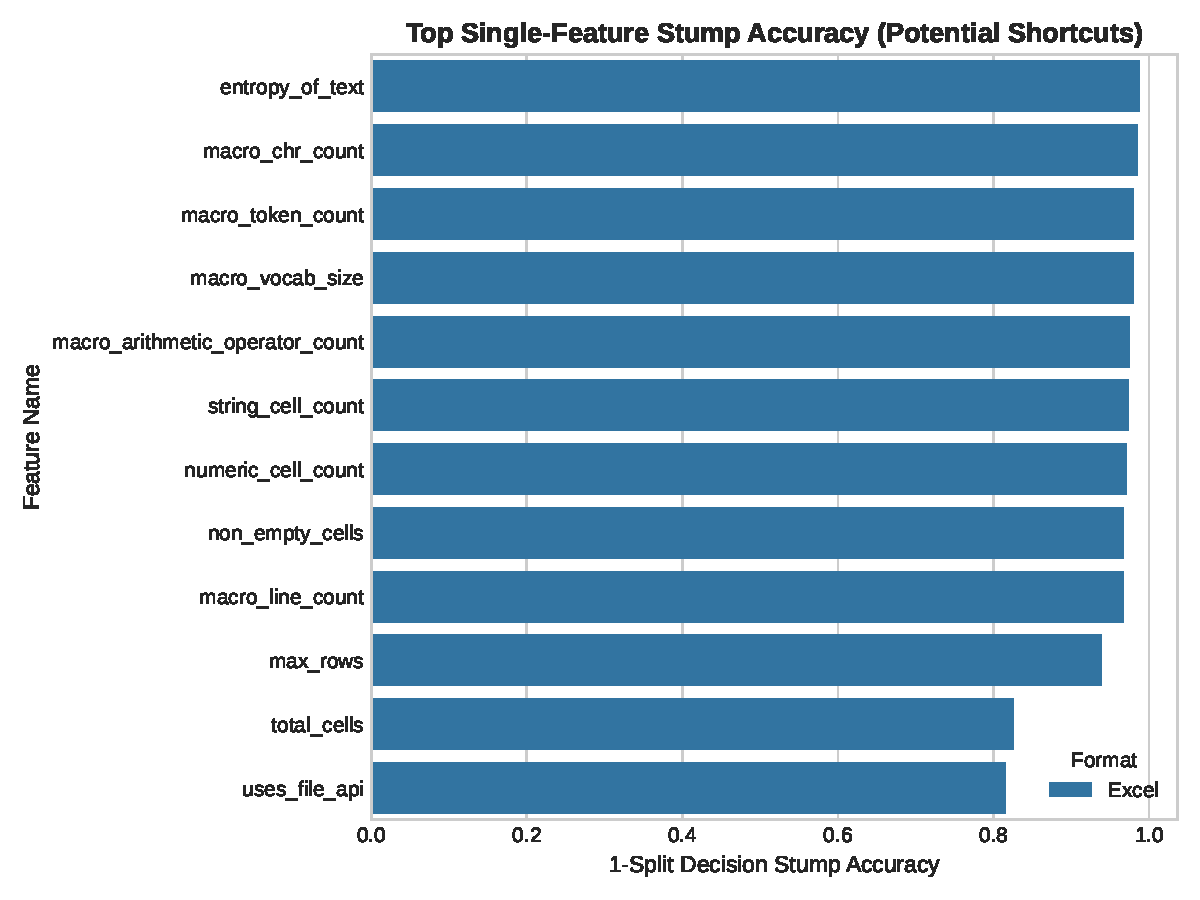
\includegraphics[width=0.84\columnwidth]{figures/fig2_stump_auc_top_features.pdf}
\caption{Twelve highest single-feature stump accuracies for Excel (\texttt{audit\_shortcuts.csv}); nine columns reach 0.95 or more, the top five being 0.987--0.975. No PDF or HTML column reaches 0.95, so only Excel is shown.}
\label{fig:stump}
\end{figure}

\begin{figure}[t]
\centering
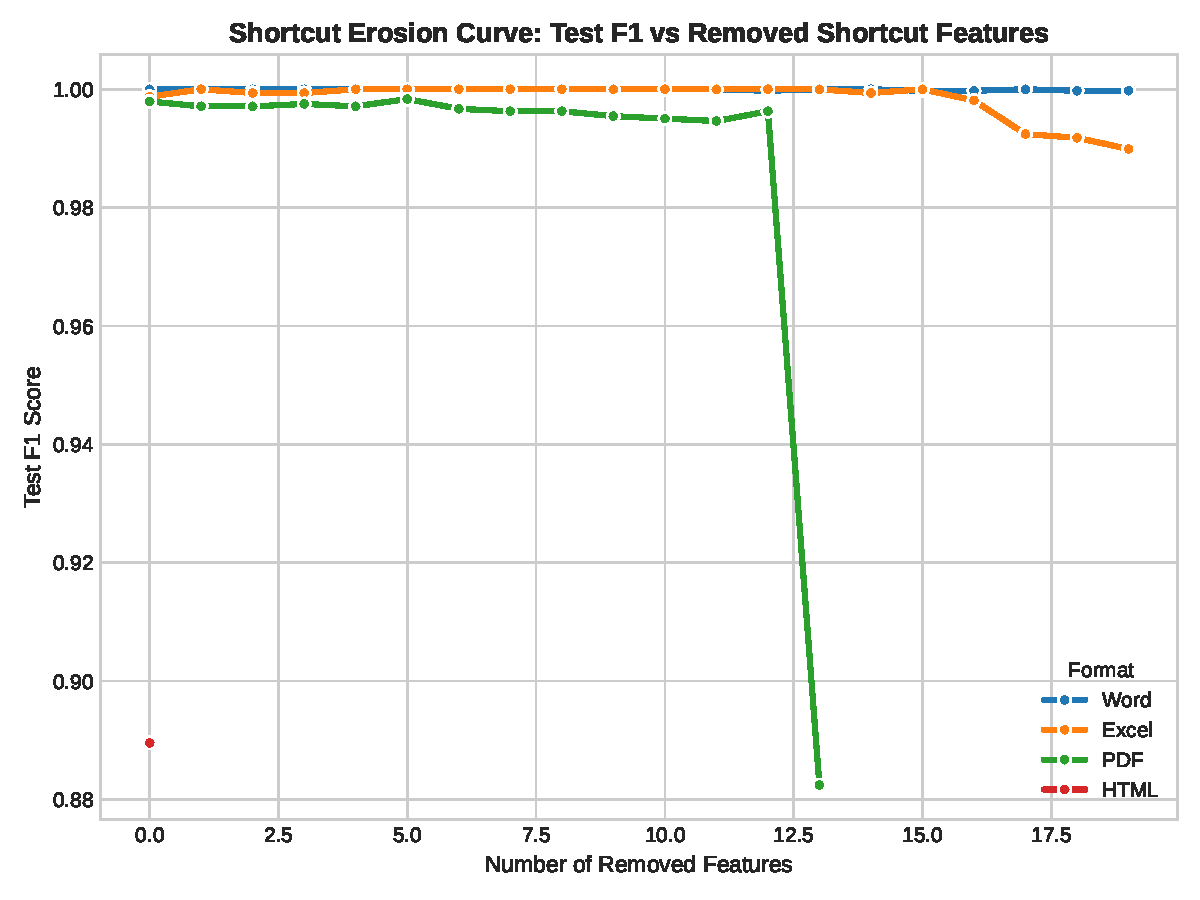
\includegraphics[width=0.84\columnwidth]{figures/fig4_shortcut_erosion_curves.pdf}
\caption{Test F1 versus number of removed features (\texttt{shortcut\_erosion\_curve.csv}), using a default (untuned) LightGBM at L1 and removing features in order of 5-fold stump accuracy. The loop stops once F1 falls below 0.90: HTML starts at 0.8896 and so has a single point, and PDF stops at 0.8824 after 13 removals (from 0.9979 at the start). Word stays at or above 0.9997 and Excel at or above 0.9899 after 19 removals.}
\label{fig:erosion}
\end{figure}

\subsection{Honest leaderboard}
Table~\ref{tab:lb} and Fig.~\ref{fig:levels} give test F1 at the three levels. At L1, Word is 1.0000, Excel 0.9993 [0.9979, 1.0000], PDF 0.9974 [0.9955, 0.9989] and HTML 0.9276 [0.9178, 0.9375]. The only large change appears in Word at L2 (0.9366 [0.9292, 0.9448]) and a small one in Excel (0.9989 [0.9977, 1.0000]); PDF and HTML are unchanged at L2 because no shortcut was flagged. Hypothesis H1 (deduplication lowers test metrics in every format) is \emph{not supported}: Word is unchanged, and HTML F1 moves from 0.9187 to 0.9276 (Table~\ref{tab:hyp}). The L0 and L1 test sets differ, duplicates are label-skewed, and tuning adds noise, so L0 and L1 scores are not like-for-like. Evidence for leakage therefore rests on the twin versus non-twin comparison below, not on the L0$\to$L1 change.

\begin{table*}[t]
\centering\footnotesize
\caption{Honest leaderboard: test F1 with 95\% bootstrap CI for the tuned LightGBM specialist (\texttt{honest\_leaderboard.csv}). L0 uses all rows; L1 and L2 are deduplicated; L2 also removes shortcut and missing-value columns (PDF and HTML: no column flagged, so L2 equals L1).}
\label{tab:lb}
\begin{tabular}{lllllll}
\toprule
Level & Format & F1 & 95\% CI & Acc. & Prec. & Rec. \\
\midrule
L0 & Word & 1.0000 & [1.0000, 1.0000] & 1.0000 & 1.0000 & 1.0000 \\
L0 & Excel & 1.0000 & [1.0000, 1.0000] & 1.0000 & 1.0000 & 1.0000 \\
L0 & PDF & 0.9988 & [0.9978, 0.9997] & 0.9987 & 0.9985 & 0.9990 \\
L0 & HTML & 0.9187 & [0.9096, 0.9272] & 0.9175 & 0.9057 & 0.9320 \\
\midrule
L1 & Word & 1.0000 & [1.0000, 1.0000] & 1.0000 & 1.0000 & 1.0000 \\
L1 & Excel & 0.9993 & [0.9979, 1.0000] & 0.9993 & 0.9985 & 1.0000 \\
L1 & PDF & 0.9974 & [0.9955, 0.9989] & 0.9974 & 0.9974 & 0.9974 \\
L1 & HTML & 0.9276 & [0.9178, 0.9375] & 0.9276 & 0.9243 & 0.9309 \\
\midrule
L2 & Word & 0.9366 & [0.9292, 0.9448] & 0.9401 & 0.9859 & 0.8920 \\
L2 & Excel & 0.9989 & [0.9977, 1.0000] & 0.9989 & 1.0000 & 0.9978 \\
L2 & PDF & 0.9974 & [0.9955, 0.9989] & 0.9974 & 0.9974 & 0.9974 \\
L2 & HTML & 0.9276 & [0.9178, 0.9375] & 0.9276 & 0.9243 & 0.9309 \\
\bottomrule
\end{tabular}
\end{table*}

\begin{figure}[t]
\centering
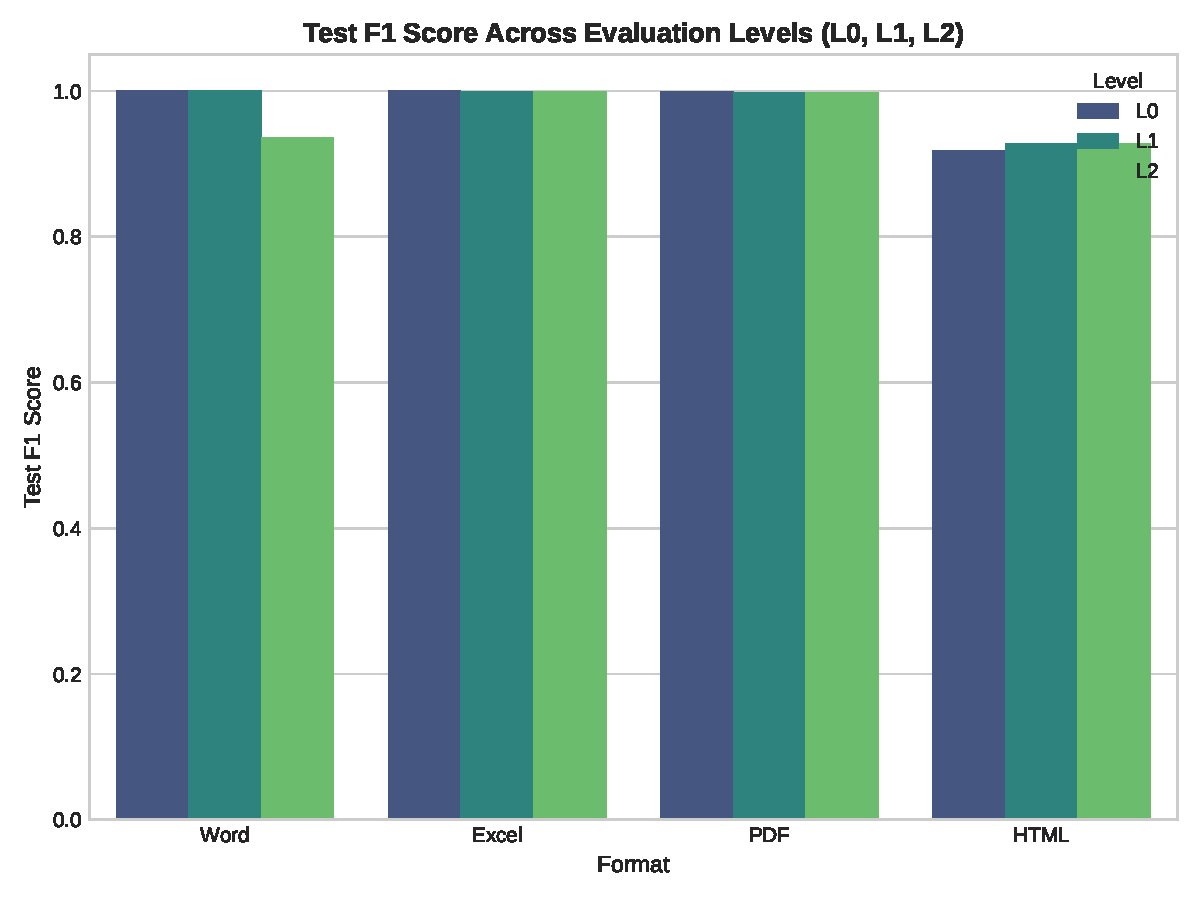
\includegraphics[width=0.84\columnwidth]{figures/fig5_l0_l1_l2_grouped_bars.pdf}
\caption{Test F1 per format at L0, L1 and L2 (\texttt{honest\_leaderboard.csv}). Word drops from 1.0000 to 0.9366 at L2; HTML is 0.9187 (L0) and 0.9276 (L1, L2). The figure has no error bars; 95\% intervals are in Table~\ref{tab:lb}.}
\label{fig:levels}
\end{figure}

\subsection{Twin versus non-twin}
Table~\ref{tab:twin} and Fig.~\ref{fig:twin} compare accuracy and F1 on L0 test rows. For HTML, twin rows ($n=1{,}083$) reach accuracy 0.9741 and F1 0.9860 [0.9804, 0.9909], while non-twin rows ($n=2{,}917$) reach accuracy 0.9009 and F1 0.8566 [0.8402, 0.8731]; the intervals do not overlap. PDF is 1.0000 on twin rows and 0.9982 on non-twin rows. Excel and Word are saturated; Word twin rows contain no positive class, so we report accuracy rather than F1 for them. The twin analysis refits the tuned LightGBM with missing values set to 0; on HTML it classifies 3,683 of 4,000 rows correctly (0.921), versus 0.9175 in Table~\ref{tab:lb}, while for PDF the two agree (0.9987).

\begin{table*}[t]
\centering\footnotesize
\caption{Twin versus non-twin L0 test rows (\texttt{twin\_vs\_nontwin.csv}). For Word, twin rows contain no positive class, so only accuracy is meaningful.}
\label{tab:twin}
\begin{tabular}{lrrlrrl}
\toprule
 & \multicolumn{3}{c}{Twin rows} & \multicolumn{3}{c}{Non-twin rows} \\
\cmidrule(lr){2-4}\cmidrule(lr){5-7}
Format & $n$ & Acc. & F1 [95\% CI] & $n$ & Acc. & F1 [95\% CI] \\
\midrule
Word & 834 & 1.0000 & n/a (no positives) & 3,166 & 1.0000 & 1.0000 [1.0000, 1.0000] \\
Excel & 1,314 & 1.0000 & 1.0000 [1.0000, 1.0000] & 2,686 & 1.0000 & 1.0000 [1.0000, 1.0000] \\
PDF & 1,074 & 1.0000 & 1.0000 [1.0000, 1.0000] & 2,786 & 0.9982 & 0.9973 [0.9947, 0.9995] \\
HTML & 1,083 & 0.9741 & 0.9860 [0.9804, 0.9909] & 2,917 & 0.9009 & 0.8566 [0.8402, 0.8731] \\
\bottomrule
\end{tabular}
\end{table*}

\begin{figure}[t]
\centering
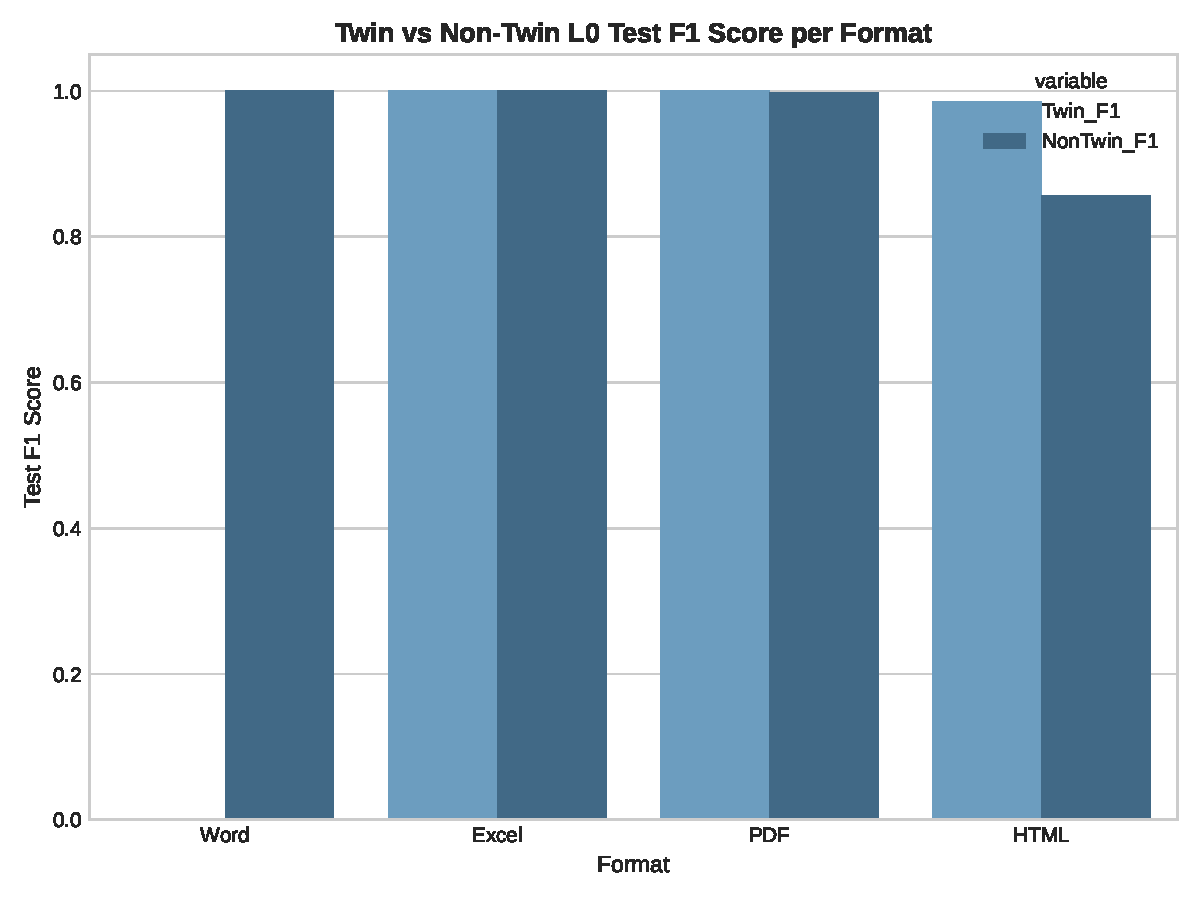
\includegraphics[width=0.84\columnwidth]{figures/fig1_duplicate_twin_leakage.pdf}
\caption{Test F1 on twin and non-twin L0 test rows (\texttt{twin\_vs\_nontwin.csv}). HTML: 0.9860 (twin) versus 0.8566 (non-twin). The Word twin bar is absent because twin rows contain no positive class (F1 undefined; accuracy 1.0000). Twin shares are in Table~\ref{tab:audit}.}
\label{fig:twin}
\end{figure}

\subsection{Word and Excel controls}
Table~\ref{tab:ctrl} gives the controls. With only the two surviving Word features, F1 is 0.9366 (accuracy 0.9401, precision 0.9859, recall 0.8920; 21 false positives and 178 false negatives on 3,321 test rows), identical to the L2 result: the residual signal is real but much weaker than the 1.000 obtained with the shortcut columns. For Excel, removing all macro and API columns still gives F1 1.0000 [1.0000, 1.0000] on 2,795 test rows (26 of 48 columns remain after removing the 22 macro and API columns). Because benign Excel files were generated synthetically \cite{nejati2026} and malicious ones are real malware, we interpret this as separability by file generation and provenance rather than by content, so Excel is not informative as a content-based benchmark. Likewise, Word is separable through missing-value patterns and OLE/VBA counts, which may reflect collection artifacts.

\begin{table}[t]
\centering\footnotesize
\caption{Controls (\texttt{control\_experiments.csv}; L1 rows from \texttt{honest\_leaderboard.csv}). Test F1 with 95\% CI.}
\label{tab:ctrl}
\begin{tabular}{p{2.6cm}lll}
\toprule
Setting & F1 & 95\% CI & Acc. \\
\midrule
Word, all columns (L1) & 1.0000 & [1.0000, 1.0000] & 1.0000 \\
Word, 2 clean features & 0.9366 & [0.9292, 0.9448] & 0.9401 \\
Excel, all columns (L1) & 0.9993 & [0.9979, 1.0000] & 0.9993 \\
Excel, no macro/API cols. & 1.0000 & [1.0000, 1.0000] & 1.0000 \\
\bottomrule
\end{tabular}
\end{table}

\subsection{Universal features}
Table~\ref{tab:uni} reports $\Delta F1$ for per-format universal models at $k=4,6,8,10$ and for the pooled model, and Fig.~\ref{fig:forest} and Fig.~\ref{fig:sens} plot them.

\textbf{Excel and PDF.} Excel shows no gap (per-format $-0.0007$ [$-0.0019$, 0.0000] at every $k$; pooled 0.0000 [$-0.0015$, 0.0015]). PDF gaps are small: 0.0116, 0.0038, 0.0019 and 0.0025 at $k=4,6,8,10$ (the $k=8$ interval includes 0), and 0.0093 [0.0059, 0.0131] pooled (Holm-adjusted $p=1.8\times10^{-4}$).

\textbf{HTML.} The pooled HTML gap is 0.0731 [0.0605, 0.0853] (Cohen's $d=12.2$). The per-format gap falls steadily from 0.0696 [0.0601, 0.0854] at $k=4$ to 0.0384 [0.0307, 0.0533] at $k=10$, a slope of $-0.004995$ per feature (H5). The gap is not shown to plateau within $k\le10$, so we do not conclude that HTML inherently needs bespoke features.

\textbf{Word.} We report two variants. With shortcut-bearing adapters, 7 of the 9 non-constant Word slots depend on columns that L2 removes (e.g., \ft{ole_object_count}, \ft{vba_keywords_count}, \ft{entropy}, \ft{file_size}; derived from \ft{mapping_log.json} and \ft{l2_removed_features.csv}); the per-format gap is 0.0000 at all $k$ with both F1 values at 1.0000. With shortcut-free adapters (``Word (No Shortcuts)'' in the results file; specialist F1 0.9366), only the two surviving columns enter the adapter (\ft{struct_script} in slots 2 and 10, \ft{struct_typeface} in slots 5 and 7) and all other slots are the constant 0. At $k=4$ a single informative feature remains (\ft{struct_script}$>0$) and the per-format gap is 0.1578 [0.1432, 0.1746]; from $k=6$ both surviving columns are present and the gap is 0.0000, consistent with the adapter and the L2 specialist using the same information. The pooled model uses the shortcut-free Word adapter: its Word F1 is 0.3047 against the L2 specialist's 0.9366, a gap of 0.6319 [0.6085, 0.6540]. Because four of its six Word slots are constant, this gap mainly shows that the two remaining Word columns carry little signal once mapped into slots shared with the other formats. The pooled Word gap is not significant under the corrected resampled $t$-test ($t=0.91$, Holm-adjusted $p=0.659$) although McNemar's test and the bootstrap interval indicate a large gap, so we treat it as indicative only. Apparent universality on Word therefore came from shortcut features.

\begin{table*}[t]
\centering\scriptsize\setlength{\tabcolsep}{3pt}
\caption{Universal-feature gap $\Delta F1$ = specialist F1 $-$ universal F1, with 95\% bootstrap CI (\texttt{sensitivity\_k.csv}; pooled column from \texttt{transfer\_gap\_significance.csv}). Per-format columns use slots 1 to $k$. The pooled model is a single LightGBM trained on all four formats with the first six slots ($k=6$); its Word row uses the shortcut-free adapters (specialist L2 F1 0.9366, universal F1 0.3047). Specialist: tuned LightGBM at L1, except ``Word (no shortcuts)'' (L2, F1 0.9366).}
\label{tab:uni}
\resizebox{\textwidth}{!}{%
\begin{tabular}{llllll}
\toprule
Format & $k=4$ & $k=6$ & $k=8$ & $k=10$ & Pooled \\
\midrule
Word (shortcut-bearing) & 0.0000 [0.0000, 0.0000] & 0.0000 [0.0000, 0.0000] & 0.0000 [0.0000, 0.0000] & 0.0000 [0.0000, 0.0000] & -- \\
Word (no shortcuts) & 0.1578 [0.1432, 0.1746] & 0.0000 [0.0000, 0.0000] & 0.0000 [0.0000, 0.0000] & 0.0000 [0.0000, 0.0000] & 0.6319 [0.6085, 0.6540] \\
Excel & $-$0.0007 [$-$0.0019, 0.0000] & $-$0.0007 [$-$0.0019, 0.0000] & $-$0.0007 [$-$0.0019, 0.0000] & $-$0.0007 [$-$0.0019, 0.0000] & 0.0000 [$-$0.0015, 0.0015] \\
PDF & 0.0116 [0.0079, 0.0159] & 0.0038 [0.0013, 0.0065] & 0.0019 [$-$0.0006, 0.0045] & 0.0025 [0.0003, 0.0051] & 0.0093 [0.0059, 0.0131] \\
HTML & 0.0696 [0.0601, 0.0854] & 0.0553 [0.0469, 0.0707] & 0.0490 [0.0410, 0.0631] & 0.0384 [0.0307, 0.0533] & 0.0731 [0.0605, 0.0853] \\
\bottomrule
\end{tabular}}
\end{table*}

\begin{figure}[t]
\centering
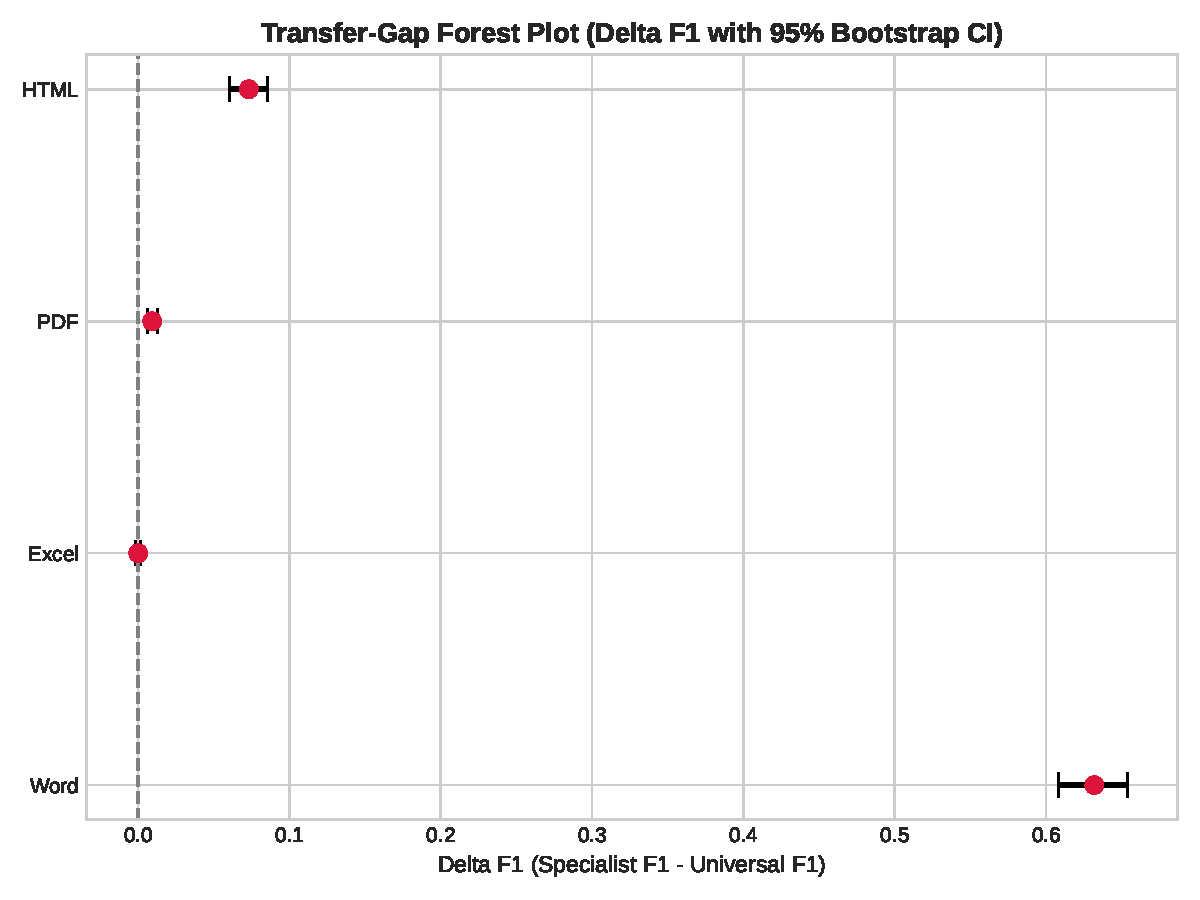
\includegraphics[width=0.84\columnwidth]{figures/fig11_transfer_gap_forest.pdf}
\caption{Pooled transfer gap $\Delta F1$ (specialist minus universal) with 95\% bootstrap CIs (\texttt{transfer\_gap\_significance.csv}): Word 0.6319, Excel 0.0000, PDF 0.0093, HTML 0.0731. Word's adapter definition is given in the text.}
\label{fig:forest}
\end{figure}

\begin{figure}[t]
\centering
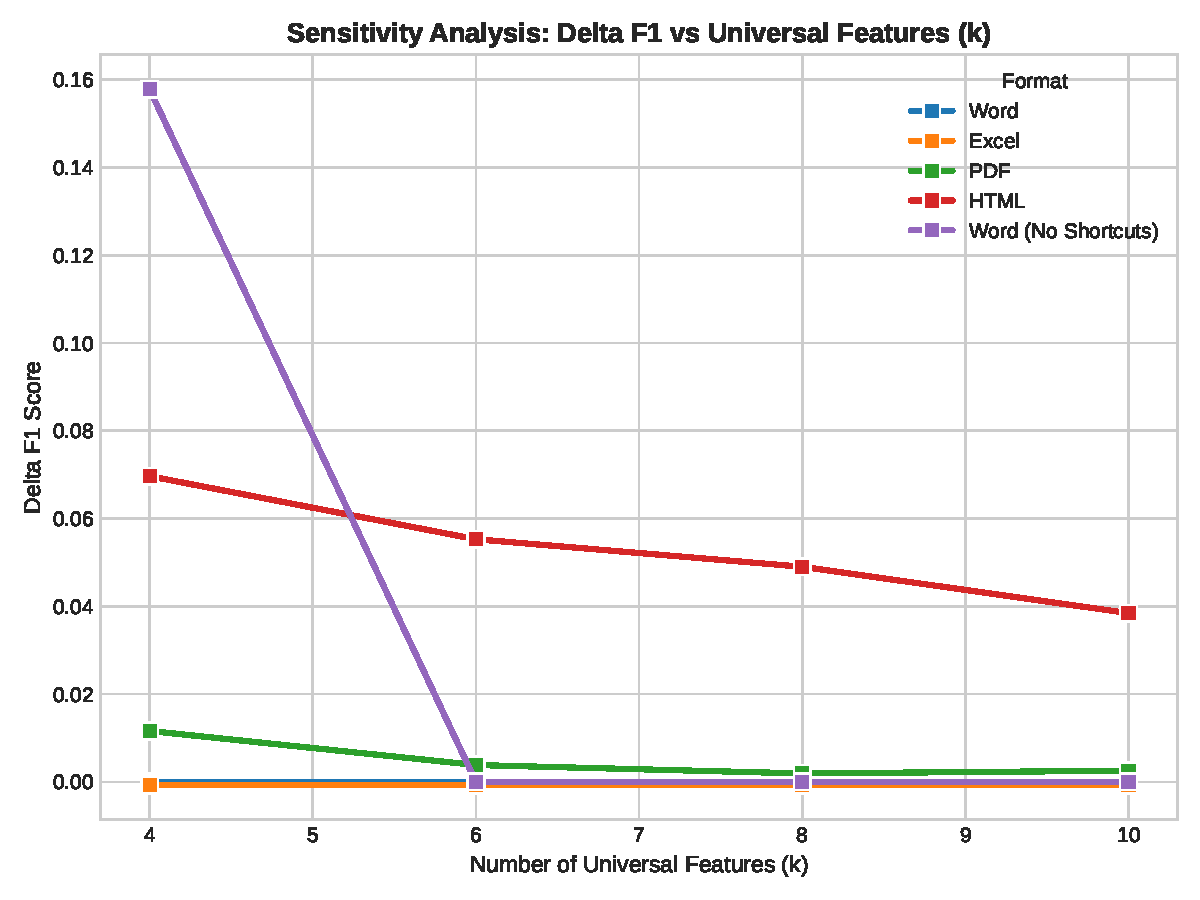
\includegraphics[width=0.84\columnwidth]{figures/fig12_sensitivity_k.pdf}
\caption{$\Delta F1$ versus feature budget $k$ (\texttt{sensitivity\_k.csv}). The HTML gap falls from 0.0696 to 0.0384; ``Word (No Shortcuts)'' falls from 0.1578 at $k=4$ to 0 at $k\ge6$; Word with shortcut-bearing adapters and Excel stay at about 0.}
\label{fig:sens}
\end{figure}

\subsection{Zero-filled union, transfer and ensembles}
\textbf{Zero-filled union.} At L1, the share of mean $|$SHAP$|$ on a row's own-format columns is 0.670 (Word), 0.621 (Excel), 0.486 (PDF) and 0.518 (HTML), so 33--51\% of attribution falls on other formats' zero-filled columns (Fig.~\ref{fig:arm4}). At L0 the own-format shares are 0.649, 0.631, 0.488 and 0.497; at L2 they are 0.388, 0.727, 0.629 and 0.576. Word's own-format share falls below 0.4 once its shortcut columns are removed. H6 (own-format columns carry at least 50\% of importance) is not supported, because PDF is below 0.5 at L0 and L1.

\begin{figure}[t]
\centering
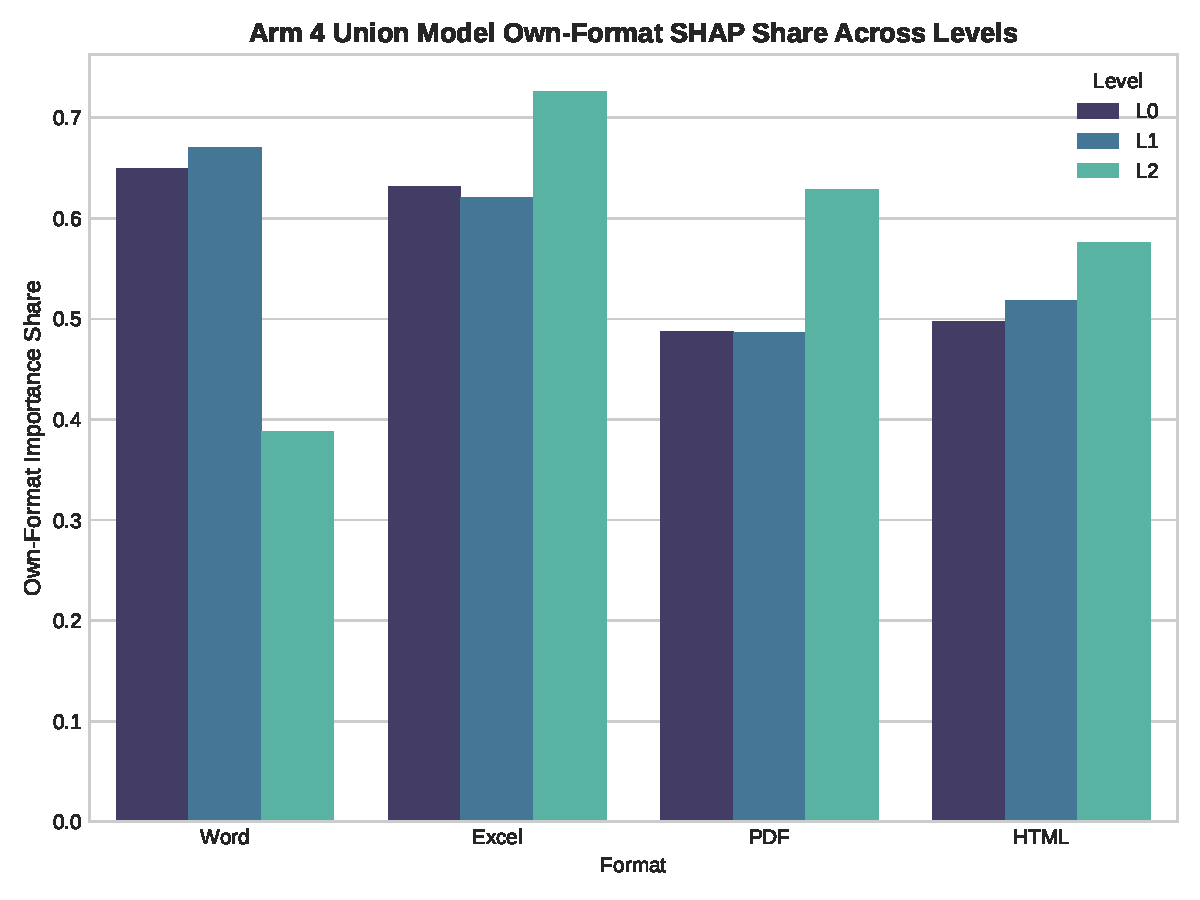
\includegraphics[width=0.84\columnwidth]{figures/fig10_arm4_shap_share.pdf}
\caption{Own-format share of mean $|$SHAP$|$ in the zero-filled union model at L0, L1 and L2 (\texttt{arm4\_shap\_share.csv}). At L1 the shares are 0.670, 0.621, 0.486 and 0.518 for Word, Excel, PDF and HTML.}
\label{fig:arm4}
\end{figure}

\textbf{Leave-one-format-out.} Training on the other three formats with the first six universal slots, transfer to an unseen format is poor: LOFO accuracy ranges from 0.130 (PDF held out) to 0.722 (Excel held out) and LOFO F1 from 0.229 (PDF) to 0.665 (Word), i.e., $\Delta F1$ against the specialists of 0.276 (HTML) to 0.769 (PDF). PDF accuracy is below chance (0.130).

\textbf{Ensembles.} Soft-voting and stacking ensembles leave Word (1.0000) and Excel (0.9993) unchanged and give PDF 0.9978. On HTML they reach 0.9366 [0.9282, 0.9453] (soft voting) and 0.9384 [0.9298, 0.9467] (stacking) versus 0.9276 [0.9178, 0.9375] for the best single model, a modest gain with overlapping intervals. We do not treat ensembles as a contribution.

\subsection{Explainability limits}
On all 223 HTML errors at L1 (117 false positives, 106 false negatives), LIME ranks \ft{mailto_link_count} first for 216 (112 and 104). The top-5 lists of TreeSHAP and permutation importance share no features; LIME's top-5 shares two with TreeSHAP and none with permutation importance. The three methods thus disagree, and the near-constant LIME top-1 suggests instability here; we do not claim that LIME identified real error causes. Error samples form three K-means clusters (silhouette 0.884). This is a negative result for explaining HTML errors with these tools.

\section{Discussion and Recommendations}
Table~\ref{tab:hyp} lists the six pre-specified hypotheses and their outcomes.

\begin{table*}[t]
\centering\footnotesize
\caption{Hypotheses and outcomes (\texttt{hypotheses.csv}). H3 holds with disjoint CIs for Word only; the Excel difference is within noise.}
\label{tab:hyp}
\begin{tabular}{lp{5.2cm}lp{6.0cm}}
\toprule
 & Hypothesis & Outcome & Evidence \\
\midrule
H1 & Deduplication lowers test metrics in every format & Not supported & Word 1.0000$\to$1.0000; Excel 1.0000$\to$0.9993; PDF 0.9988$\to$0.9974; HTML 0.9187$\to$0.9276 \\
H2 & Word and Excel each contain a feature with stump accuracy $\ge0.95$ & Supported & Word and Excel both have columns above 0.95 (Word 19, Excel 9) \\
H3 & L2 F1 is lower than L1 for Word and Excel & Supported & Word 1.0000$\to$0.9366 (CIs disjoint); Excel 0.9993$\to$0.9989 (CIs overlap) \\
H4 & Pooled universal F1 within 0.01 of the specialist for Word, Excel and PDF but not HTML & Inconclusive & PDF CI upper bound 0.0131 $>0.01$; Word 0.6319; Excel 0.0000; HTML 0.0731 \\
H5 & The HTML gap shrinks as $k$ grows & Supported & Slope of HTML $\Delta F1$ on $k$: $-0.004995$ \\
H6 & Own-format columns carry $\ge50\%$ of importance in the zero-filled union & Not supported & Own-format shares at L1: 0.670, 0.621, 0.486, 0.518 \\
\bottomrule
\end{tabular}
\end{table*}

Three patterns emerge. First, the audit finds substantial exact duplication (Table~\ref{tab:audit}), but its effect on aggregate F1 is small and not uniform; the twin/non-twin split shows where it matters (HTML). Second, Word and Excel scores are explained by shortcuts or provenance: removing them leaves Word at 0.9366 and shows Excel to be separable without any macro or API column. Third, universal features show no or small gaps on Excel and PDF, a larger gap on HTML that shrinks with $k$, and large losses on Word once shortcuts are removed.

\textbf{Checklist for benchmark builders.}
\begin{enumerate}
\item Deduplicate feature vectors \emph{before} splitting; report both rows inside duplicate groups and rows removed.
\item Report the twin share of the test set and metrics on twin and non-twin rows.
\item Release provenance metadata and test whether folder names or extensions predict the label.
\item Match benign and malicious collection pipelines; synthetic benign files make content-based claims unreliable.
\item Screen single-feature stumps and missing-value indicators; drop or justify columns above a stated threshold.
\item Report confidence intervals and the evaluation level (L0/L1/L2) with every score.
\item Do not zero-fill a union of formats without attributing importance by format.
\item Treat attribution tools as unvalidated until they agree on a task with known ground truth.
\item Release seeds, split indices and code.
\end{enumerate}

\section{Limitations and Threats to Validity}
We study static features and one benchmark release. Benign Excel files are synthetic, so Excel and Word cannot measure content-based detection. Only exact duplicates were removed; a rough near-duplicate screen (distance at most $0.1\sqrt{P}$ for $P$ columns, on standardized features with missing values imputed as $-999$ before scaling) was computed but not used and is not reported, because the imputation distorts distances. Optuna used 8 trials and 3-fold inner CV because of compute limits. The specialist is the tuned LightGBM; other families and ensembles score slightly higher on HTML (ensembles 0.9366 and 0.9384 versus 0.9276). The twin analysis refits the tuned LightGBM with missing values set to 0, so its HTML accuracy differs slightly from Table~\ref{tab:lb}. File-path provenance could not be tested for Word because the release has no path field. LIME was unreliable. There is no external dataset, temporal split or adversarial evaluation. The universal adapters are hand-designed and feature semantics differ between formats, and the L2 thresholds (stump accuracy 0.95) are a choice. Prior-work comparisons rest on published setups and are not directly comparable.

\section{Conclusion}
On CIC-Trap4Phish, exact duplicates and twin leakage are measurable in all four formats, and accuracy on non-twin HTML rows is lower than on twin rows (0.857 versus 0.986 F1). Word's saturated scores depend on shortcut and missing-value columns; the honest Word F1 is 0.937 [0.929, 0.945], and Excel's separability reflects provenance. Pooled universal features nearly match specialists on Excel and PDF but not on HTML (0.073 [0.060, 0.085]), where the per-format gap shrinks with feature budget. We encourage benchmark builders to adopt the checklist above.

\section*{Data and Code Availability}
Code, seeds (42) and split indices: {https://github.com/Atharv-K-979/FEMDoc}. The full pipeline run is recorded as complete, with a duration of about 1,788 seconds (\todo{hardware}).

\section*{Acknowledgment}
\todo{acknowledgment}

\bibliographystyle{IEEEtran}
\bibliography{references}

\end{document}
